\documentclass[compress]{beamer}

\usepackage{tikz}
\usetikzlibrary{shapes,arrows}
\usepackage{color}
\usepackage[utf8]{inputenc}
\usepackage{amssymb}
\setbeamertemplate{caption}{\raggedright\insertcaption\par}

\usetheme[navigation]{UMONS}
%\usetheme[navigation, no-subsection, no-totalframenumber]{UMONS}

\newcommand{\IR}{\mathbb{R}}


\title{Bandwidth estimation : metrics, measurement techniques, and tools}
\author{M. Lempereur \\
J. Gheysen}
\institute[(Info)]{%
  Département d'Informatique\\
  Université de Mons
  \\[2ex]
  
\includegraphics[height=4ex]{UMONS}\hspace{2em}%
  \raisebox{-1ex}{
\includegraphics[height=6ex]{UMONS_FS}}
}

\begin{document}

\begin{frame}[plain]
  \titlepage
\end{frame}

\begin{frame}
  \tableofcontents
\end{frame}

\section{Introduction}
\begin{frame}{Introduction}

\end{frame}

%%%%%%%%%%%%%%%%%%%%%%%%%%%%%%%%%%%%%%%%%%%%%%%%%%%%%%%%%%%%%%%%%%%%%%%%
%Dans l'utilisation quotidienne beaucoup de termes sont
%confondus, le but ici est de formaliser la définition autour
%de la vitesse d'une connection et de la "bande passante".
%D'apporter des mesures précises et de faire le point sur les
%technologies existantes à ce niveau. 
%%%%%%%%%%%%%%%%%%%%%%%%%%%%%%%%%%%%%%%%%%%%%%%%%%%%%%%%%%%%%%%%%%%%%%%%

\begin{frame}{Introduction}{Vocabulaire 1/2}
	\begin{figure}
   		\begin{minipage}[c]{.46\linewidth}
   			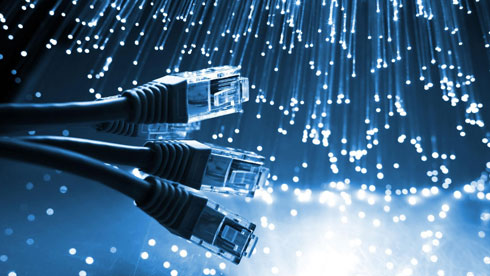
\includegraphics[scale=0.23]{capacity.jpg}
   			\caption{Capacité}
   		\end{minipage} \hfill
   		\pause
   		\begin{minipage}[c]{.46\linewidth}
      		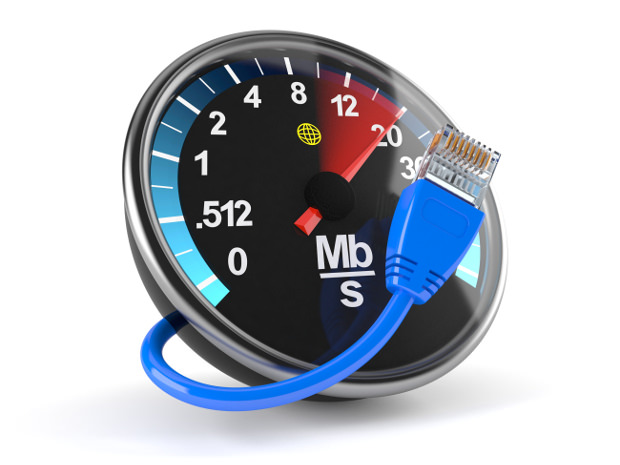
\includegraphics[scale=0.18]{bande_passante.jpg}
      		\caption{Bande Passante}
   		\end{minipage}
   		\pause
   		\begin{minipage}[c]{.46\linewidth}
   			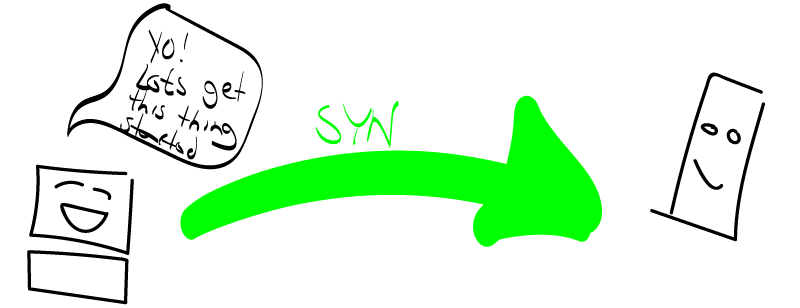
\includegraphics[scale=0.2]{tcp.png}
   			\caption{Bulk-Transfert-Capacity}
   		\end{minipage} \hfill
	\end{figure}
\end{frame}

\begin{frame}{Introduction}{Vocabulaire 2/2}
\begin{itemize}
	\item Différenciation entre liens de la couche données (1) et couche IP(2).
	\begin{enumerate}
		\item \textbf{Segment} : Lien physique point à point. %Etendre aux autres points dans l'article ?
		\item \textbf{Hop} (saut) : Consiste en un ensemble de segments. %Connectés à travers switchs/bridges...
	\end{enumerate}
	\vspace{10pt}
	\item \textbf{Chemin end-to-end} : Lie un hôte à une source via une suite de hops.
	\vspace{10pt}
	\item Que mesurer ? Dans quelle situation ? 
	\begin{itemize}
		\item \textbf{Lien unique (hop)} : Capacité, Bande Passante.
		\item \textbf{Chemin} : Capacité, Bande Passante, Bulk-Transfert-Capacity.
	\end{itemize}
\end{itemize}
\end{frame}

%%%%%%%%%%%%%%%%%%%%%%%%%%%%%%%%%%%%%%%%%%%%%%%%%%%%%%%%%%%%%%%%%%%%%%%%
%Tout d'abord != entre lien et chemin (= ensemble de liens)
%ATTENTION : UN SEGMENT est en réalité une FRAME (layer 2).
%Ici nous utilisons lien pour donner définition globale.
%Capacité : Valeur maximale du flux pouvant traverser un lien,
%càd quantité maximale de bits pouvant transiter à travers
%le lien par unité de temps. 
%Bande passante disponible : Capacité du lien non utilisée,
%alors utilisable afin d'écouler du traffic. 
%BTC : Représente le débit atteignable par une seule 
%connexion TCP. 
%%%%%%%%%%%%%%%%%%%%%%%%%%%%%%%%%%%%%%%%%%%%%%%%%%%%%%%%%%%%%%%%%%%%%%%%


\section{Données mesurées}
\subsection{Capacité}
\begin{frame}{Capacité}
	Posons :
	\begin{itemize}
	\item $C_{L2}$ la capacité nominale du \textbf{segment},
	\item $L_{L3}$ la taille du paquet IP, 
	\item $H_{L2}$ l'overhead de la couche 2. 
	\end{itemize}
	\begin{block}{Temps de transmission : $\Delta_{L3}$}
		$$\Delta_{L3} = \frac{L_{L3} + H_{L2}}{C_{L2}}$$
	\end{block}
	\begin{block}{Capacité couche IP:  $C_{L3}$}
		$$C_{L3} = \frac{L_{L3}}{\Delta_{L3}} = \frac{L_{L3}}{\frac{L_{L3}+H_{L2}}{C_{L2}}} = C_{L2} \frac{1}{1+\frac{H_{L2}}{L_{L3}}}$$
	\end{block}
\end{frame}
%%%%%%%%%%%%%%%%%%%%%%%%%%%%%%%%%%%%%%%%%%%%%%%%%%%%%%%%%%%%%%%%%%%%%%%%
%Bien insister sur le fait qu'on regarde le paquet IP au 
%travers d'un SEGMENT. 
%La capacité C_L3 est donc directement proportionnelle à la 
%capacité de la couche d'en dessous et inversément proportionnelle
%au rapport Overhead/Longueur (Plus ce rapport est grand plus la 
%capacité est réduite. Ce dernier dépend du MTU (Maximum Transfert
%Unit) d'un paquet de la couche IP. 
%%%%%%%%%%%%%%%%%%%%%%%%%%%%%%%%%%%%%%%%%%%%%%%%%%%%%%%%%%%%%%%%%%%%%%%%

\begin{frame}
	\begin{alertblock}{Remarque}
		Le rapport $\frac{H_{L2}}{L_{L3}}$ est borné par le MTU (Maximum Transmission Unit).
	\end{alertblock}
\begin{figure}[hbtp]
\centering
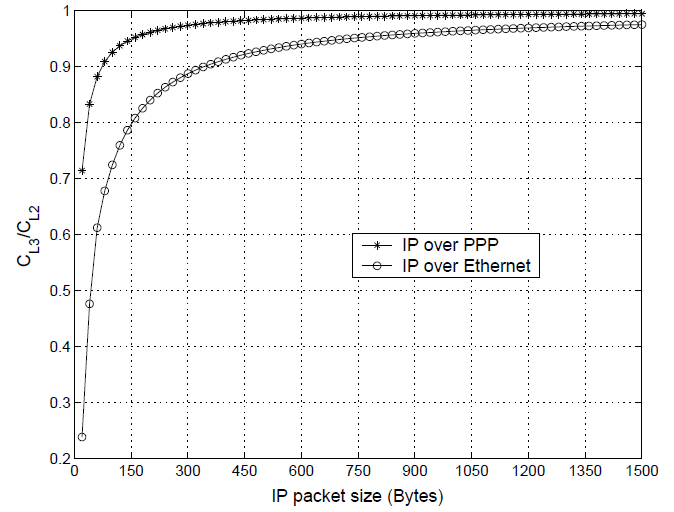
\includegraphics[scale=0.25]{schema1.PNG}
\caption{Rapport des capacités d'un segment délivré à la couche IP en fonction de sa taille.}
\end{figure}
		\begin{block}{Capacité sur un chemin}
		$$C = \min\limits_{i=1,...,H} C_{i}$$
		\end{block}
\end{frame}

%%%%%%%%%%%%%%%%%%%%%%%%%%%%%%%%%%%%%%%%%%%%%%%%%%%%%%%%%%%%%%%%%%%%%%%%
%En ce qui concerne le MTU : il définit un overhead fixe pour 
%une taille de paquet maximum => Remplir un max les paquets.
%Appelés datagrammes IP.
%Plus le paquet sera grand, plus le rapport sera petit et avantageux.   
%%%%%%%%%%%%%%%%%%%%%%%%%%%%%%%%%%%%%%%%%%%%%%%%%%%%%%%%%%%%%%%%%%%%%%%%

\subsection{Bande Passante}
\begin{frame}{Bande Passante}
	\begin{figure}[hbtp]
		\centering
		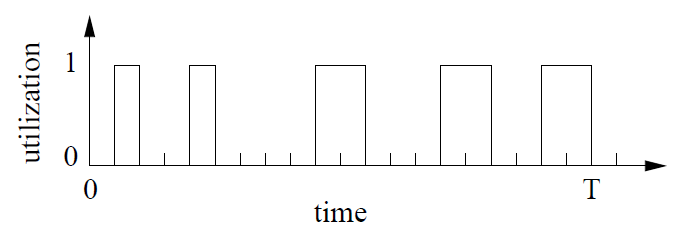
\includegraphics[scale=0.42]{schema2.PNG}
		\caption{Utilisation instantanée d'un lien durant un temps (0,T)}
	\end{figure}
	\begin{itemize}
		\item Utilisation du lien non-constante,
		\item Posons $u_i$ l'utilisation moyenne. 
	\end{itemize}
	\begin{block}{Bande passante disponible en moyenne : $A_{i}$}
		$$ A_i = (1 - u_i) C_i $$
	\end{block}
\end{frame}

%%%%%%%%%%%%%%%%%%%%%%%%%%%%%%%%%%%%%%%%%%%%%%%%%%%%%%%%%%%%%%%%%%%%%%%%
%A un temps donné, le lien transmet un paquet à sa full capacité (1) ou 
%est inutilisé. La formule donnée pour A_i comprend la bande passante 
%pour un seul hop i. 
%%%%%%%%%%%%%%%%%%%%%%%%%%%%%%%%%%%%%%%%%%%%%%%%%%%%%%%%%%%%%%%%%%%%%%%%

\begin{frame}
	\begin{block}{Bande passante sur un chemin}
		$$A = \min\limits_{i=1,...,H} A_{i}$$
	\end{block}
	\begin{alertblock}{Remarque}
		Bande passante et capacité ne sont pas toujours limitées sur le même lien. 
	\end{alertblock}
	\begin{figure}[hbtp]
		\centering
		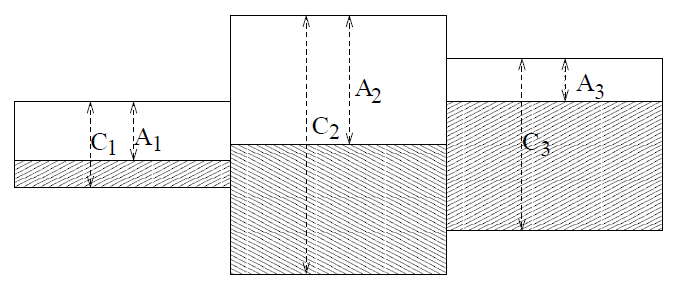
\includegraphics[scale=0.42]{schema3.PNG}
		\caption{Exemple de trafic pour un chemin de 3 hops}
	\end{figure}
	
\end{frame}

%%%%%%%%%%%%%%%%%%%%%%%%%%%%%%%%%%%%%%%%%%%%%%%%%%%%%%%%%%%%%%%%%%%%%%%%
%La bande passante disponible sur un chemin est le minimum de celle 
%dispo sur tous les liens de son chemin. 
%Dans l'exemple, la limitation se fait en 1 pour la capacité et en 3
%pour la bande passsante. 
%Ces calculs supposent que l'utilisation des liens est constante,
%cette assomption reste raisonnable pour des intervalles de temps 
%cours mais /!\ à la sporadicité et à la != diurne/nocturne, etc...
%Or ce n'est pas le cas, il faut donc effectuer des mesures rapides
%si on veut un aperçu en temps réel (utile pour certaines applis). 
%%%%%%%%%%%%%%%%%%%%%%%%%%%%%%%%%%%%%%%%%%%%%%%%%%%%%%%%%%%%%%%%%%%%%%%%

\subsection{Bulk-Transfert-Capacity}
\begin{frame}{Bulk-Transfert-Capacity (BTC)}
	\begin{alertblock}{Définition}
		Débit atteignable par une unique connection TCP en prenant compte du contrôle de congestion.
	\end{alertblock}
	Éléments influençant le flux TCP : 
	\begin{itemize}
		\item Taille des paquets transférés,
		\item Trafic croisé avec d'autres connections,
		\item Taille des buffers des sockets,
		\item Taille de la fenêtre de congestion,
		\item ...
	\end{itemize}
\end{frame}

%%%%%%%%%%%%%%%%%%%%%%%%%%%%%%%%%%%%%%%%%%%%%%%%%%%%%%%%%%%%%%%%%%%%%%%%
%Représente 90% du trafic
%Beaucoup de facteurs influençant : transfert size, cross-traffic, 
%competiting TCP connections, TCP socket buffer size, congestion, 
%variations liées à l'implémentation,...
%Pour une page Web : congestion window, RTT, slow-start mechanism
%TODO Regarder avec l'histoire de capacité C/2. 
%%%%%%%%%%%%%%%%%%%%%%%%%%%%%%%%%%%%%%%%%%%%%%%%%%%%%%%%%%%%%%%%%%%%%%%%

\section{Techniques de mesure}
\subsection{Variable Packet Size (VPS) probing}
%%%%%%%%%%%%%%%%%%%%%%%%%%%%%%%%%%%%%%%%%%%%%%%%%%%%%%%%%%%%%%%%%%%%%%%%
%Préliminaire : Pour toutes les techniques de mesure présentées, on 
%suppose que la charge du trafic est stationnaire et que la  route
%ne change pas.
%%%%%%%%%%%%%%%%%%%%%%%%%%%%%%%%%%%%%%%%%%%%%%%%%%%%%%%%%%%%%%%%%%%%%%%%
\begin{frame}{Variable Packet Size (VPS) probing}{Principe}
\begin{itemize}
\pause 
\item \textbf{But :}  Mesurer la {\color{red}capacité} de chaque saut le long d'un chemin.
\pause
\item \textbf{Idée :}  Mesurer le {\color{red}RTT} (Round-Trip-Time) de la source jusque chaque saut.
\pause
\item \textbf{Technique :} Envoyer des paquets tests avec des {\color{red}TTL} (Time-To-Live) calculés pour expirer à un saut particulier. 
\end{itemize}

%\vspace{1cm}
%
%\tikzset{node/.style={draw,ellipse,minimum width=5pt, minimum height=1.2cm, fill=black!25}}
%\begin{tikzpicture}
%	\node[node](S)at(0,0){Source};
%	\node[node](Hf)at(3,0){Hop1};
%	\node[node](Hs)at(6,0){Hop2};
%	\node[node](D)at(9,0){Destination};
%	
%	\path[->, line width=1.2pt, blue] (S) edge[bend left=20] (Hf);
%	\path[->, line width=1.2pt, blue] (Hf) edge[bend left=20] (Hs);
%	\path[->, line width=1.2pt, blue] (Hs) edge[bend left=20] (D);
%	
%	\path[->, line width=1.2pt, red] (S) edge[bend left=40] (Hf);
%	\path[->, line width=1.2pt, red] (Hf) edge[bend left=40] (Hs);
%
%	\path[->, line width=1.5pt, green] (S) edge[bend left=60] (Hf);
%\end{tikzpicture}

\end{frame}

%%%%%%%%%%%%%%%%%%%%%%%%%%%%%%%%%%%%%%%%%%%%%%%%%%%%%%%%%%%%%%%%%%%%%%%%
%Envoi de paquets avec TTL calculés pour arriver à un saut particulier.
%Comment ? TTL s'exprime en hops donc ok !
%Réponse du hop avec message ICMP, de là on peut calculer le RTT.
%%%%%%%%%%%%%%%%%%%%%%%%%%%%%%%%%%%%%%%%%%%%%%%%%%%%%%%%%%%%%%%%%%%%%%%%

\begin{frame}{Variable Packet Size (VPS) probing}{Formalisation}
	\begin{block}{Minimum RTT : $T_i$(L)}
	$$T_{i}(L) = \alpha + \beta_{i}L \text{ où } \beta_i = \sum^{I}_{k=1} \frac{1}{C_k}$$
	\end{block}
\begin{itemize}
	\item $\alpha$ : Délai de propagation jusqu'au saut i + délai de 	sérialisation et délai de propagation de la réponse ICMP.
	\item $\beta_i$ : Pente du RTT minimum jusqu'au hop i.
\end{itemize}
\pause
\begin{block}{Capacité d'un saut i : $C_i$}
	$$ C_i = \frac{1}{\beta_i - \beta_{i-1}} $$
\end{block}
\end{frame}

%%%%%%%%%%%%%%%%%%%%%%%%%%%%%%%%%%%%%%%%%%%%%%%%%%%%%%%%%%%%%%%%%%%%%%%%
%RTT a trois composantes : 
% > Délai sérialisation = temps pour mettre le paquet sur le lien
% > Délai propagation = temps pour propager le paquet via le lien
% > Délai d'attente = temps d'attente si jamais il y a contention 
%(saturation) à l'entrée où à la sortie d'un lien. 
%Dans les calculs on envoie pas mal de paquets espérant qu'un ne 
%rencontrera pas de queuing delay. 
%/!\ Erreurs importantes possibles s'il y a des store-forward 
%layer 2 switches
%%%%%%%%%%%%%%%%%%%%%%%%%%%%%%%%%%%%%%%%%%%%%%%%%%%%%%%%%%%%%%%%%%%%%%%%

\begin{frame}{Variable Packet Size (VPS) probing}{Résultats}
	\begin{figure}[hbtp]
		\centering
		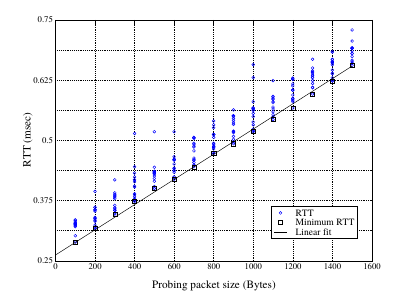
\includegraphics[scale=0.7]{schema4.png}
		\caption{Mesures de RTT pour le premier hop d'un chemin}
	\end{figure}
\end{frame}

%%%%%%%%%%%%%%%%%%%%%%%%%%%%%%%%%%%%%%%%%%%%%%%%%%%%%%%%%%%%%%%%%%%%%%%%
%On peut voir sur ce schéma la mesure des RTT, minimum RTT et la 
%droite "fittant les minimums  RTT".
%%%%%%%%%%%%%%%%%%%%%%%%%%%%%%%%%%%%%%%%%%%%%%%%%%%%%%%%%%%%%%%%%%%%%%%%

\subsection{Packet Pair/Train Dispersion (PPTD) probing}
\begin{frame}{Packet Pair/Train Dispersion (PPTD) probing}{Principe 1/3}
\begin{itemize}
	\item \textbf{But :} Mesurer la {\color{red}capacité} sur l'entièreté d'un chemin. 
	\pause
	\item \textbf{Idée :} Envoyer des {\color{red}paires de paquets} et calculer la distance en temps (dispersion) entre le dernier bit de ces derniers. 
	\begin{figure}[hbtp]
		\centering
		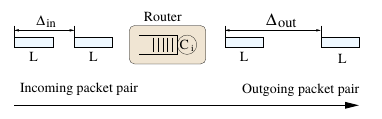
\includegraphics[scale=0.6]{schema5.png}
		\caption{Dispersion d'une paire de paquets}
	\end{figure}
	\item Dispersion résultante d'un saut : $\Delta_{out} = max (\Delta_{in} , \frac{L}{C_i})$
	\item Dispersion sur un chemin : $\Delta_R = \max\limits_{i=0,...,H} (\frac{L}{C_i}) = \frac{L}{min_{i=0,..,H}C_i} = \frac{L}{C}$
\end{itemize}
\end{frame}

%%%%%%%%%%%%%%%%%%%%%%%%%%%%%%%%%%%%%%%%%%%%%%%%%%%%%%%%%%%%%%%%%%%%%%%%
%La distance en temps entre les paquets est appelée dispersion.
%En effet la dispersion sortante = max entre celle d'entrée et celle 
%engendrée par le hop traversé. 
%De la dernière formule on déduit que C = L/DeltaR.
%%%%%%%%%%%%%%%%%%%%%%%%%%%%%%%%%%%%%%%%%%%%%%%%%%%%%%%%%%%%%%%%%%%%%%%%

\begin{frame}{Packet Pair/Train Dispersion (PPTD) probing}{Principe 2/3}
\begin{itemize}
	\item \textbf{Problème :} Il faut en réalité tenir compte du {\color{red}trafic} pouvant {\color{red}perturber} les mesures.
	\pause
	\item \textbf{Solution 1:} Envoyer un {\color{red}grand nombre} de paquet et établir des statistiques.
	\item \textbf{Résultat :} Interprétations statistiques classiques offrent des résultats peu fiables. 
	\begin{figure}[hbtp]
		\centering
		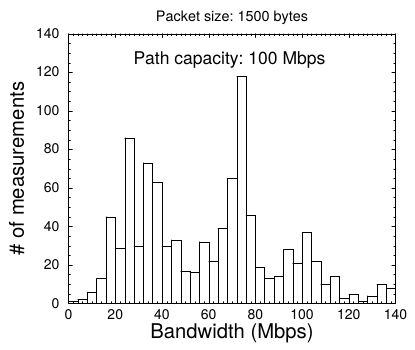
\includegraphics[scale=0.4]{schema6.png}
		\caption{Histogramme de mesures de capacité de 1000 échantillons}
	\end{figure}
\end{itemize}
\end{frame}

%%%%%%%%%%%%%%%%%%%%%%%%%%%%%%%%%%%%%%%%%%%%%%%%%%%%%%%%%%%%%%%%%%%%%%%%
%Si question, qu'engendrent perturbations de trafic ? 
% > Sous-estimation : Des paquets s'intercalent, augmentant la dispers.
% > Sur-estimation : Le premier paquet est retardé et le second non. 
% Exemple frappant sur l'histogramme, on voit que la capacité réelle de
% 100Mps est sous-estimée (probablement à cause du trafic). 
%%%%%%%%%%%%%%%%%%%%%%%%%%%%%%%%%%%%%%%%%%%%%%%%%%%%%%%%%%%%%%%%%%%%%%%%

\begin{frame}{Packet Pair/Train Dispersion (PPTD) probing}{Principe 3/3}
\begin{itemize}
	\item \textbf{Solution 2 :} Envoyer un {\color{red}train de N paquets}.
\end{itemize}
	\begin{block}{Taux de dispersion sans trafic extérieur}
		$$ D = \frac{(N-1)L}{\Delta_R(N)}$$
	\end{block}
Exemple :
\begin{itemize}
\item Chemin de deux hops avec $C_1 < C_0$
\item {\color{red}Trafic extérieur} de taux $R_C < C_1 < C_0$ sur 2\textsuperscript{ème} lien
\end{itemize} 
\vspace{10pt}
		$$ E[D] = \frac{(N-1)L}{\Delta_2} =  \frac{C_1}{1+\frac{R_C}{C_0}} < C_1$$

\end{frame}

%%%%%%%%%%%%%%%%%%%%%%%%%%%%%%%%%%%%%%%%%%%%%%%%%%%%%%%%%%%%%%%%%%%%%%%%
%Pourquoi (N-1) pour N paquets ? Car N paquets => n-1 chemins.
%\DeltaR est la dispersion end-to-end du chemin.
%Pour un chemin sans trafic : taux de dispersion = capacité.
%Le cross traffic peut rendre D bcp plus << que C. 
%On remarque que le taux de dispersion < C_1 ce qui veut dire qu'on a 
%perdu par rapport à la capacité initiale. 
% %TODO Plus il y a de trafic moins il y a d'interférence ? 
%Attention E[D] != de la bande passante. A < E[D] ? En effet :
% A < E[D] < C1  <=> C1-R < E[D] < C1
% %TODO Discuter des calculs pour D et interpréter ce D
%%%%%%%%%%%%%%%%%%%%%%%%%%%%%%%%%%%%%%%%%%%%%%%%%%%%%%%%%%%%%%%%%%%%%%%%

\subsection{Self-Loading Periodic Streams (SLoPS)}
\begin{frame}{Self-Loading Periodic Streams (SLoPS)}{Principe 1/3}
\begin{itemize}
\item \textbf{But :}  Mesurer la {\color{red}bande passante disponible} sur l'entièreté d'un chemin.
\pause
\item \textbf{Idée :}  Envoyer un certain nombre de paquets à un taux variable. Jusqu'à ce qu'on aperçoive un délai dans la file du lien tendu sur chemin.
\pause
\item \textbf{Technique :} Pour approcher la valeur de la bande passante
disponible, on utilise un algorithme itératif proche de la recherche binaire.
\end{itemize}
\end{frame}
% Si R > A alors R_max = R
% Sinon R_min = R
% Le nouveau R = (R_max + R_min)/2
\begin{frame}{Self-Loading Periodic Streams (SLoPS)}{Principe 2/3}

SLoPS basé sur une technique très simple en quelques étapes :
\begin{itemize}
\item On envoie K paquets de taille fixe avec un taux R.
\pause
\item Le receveur nous donne la valeur du One Way Delay (OWD)
\item Si $\Delta_{OWD}$ augmente alors R $>$ A sinon R $<$ A
\pause
\item On détermine la nouvelle valeur de R.
\item On répète ces étapes jusqu'à ce que $R \approx 0.9 * A$
\end{itemize}
\end{frame}

\begin{frame}{Self-Loading Periodic Streams (SLoPS)}{Principe 3/3}

Le "One Way Delay" est provoqué par une surcharge de la file
sur le lien.

La nouvelle valeur de R est déterminée à l'aide d'un algorithme
proche de la recherche binaire.

\begin{figure}[hbtp]
		\centering
		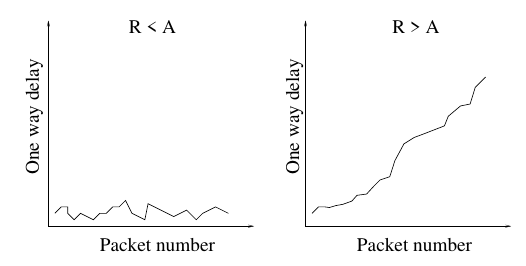
\includegraphics[scale=0.4]{slopsOWD.png}
		\caption{Évolution des OWD en fonction de R}
\end{figure}

\end{frame}

\subsection{Trains of Packet Pairs (TOPP)}
\begin{frame}{Trains of Packet Pairs (TOPP)}{Principe}
\begin{itemize}
\item \textbf{But :}  Mesurer la {\color{red}bande passante disponible} sur l'entièreté d'un chemin.
\pause
\item \textbf{Idée :}  Envoyer plusieurs paires de paquets à un taux
croissant.
\pause
\item \textbf{Technique :} On fixe un taux à l'envoi et on calcule à
nouveau le taux au niveau du receveur. Si le taux receveur $<$ taux envoi alors on a dépassé la bande passante disponible.
Sinon taux à l'entrée = taux à la sortie.
\end{itemize}
\end{frame}
\begin{frame}{Trains of Packet Pairs (TOPP)}{Principe}

TOPP et SLoPS partent de la même idée de base, ils se différencient
essentiellement sur la technique statistique des mesures ainsi que sur
l'algorithme utilisé pour trouver la nouvelle valeur du taux.
TOPP augmente de manière itérative ce taux.

TOPP a aussi l'avantage de pouvoir calculer la capacité du chemin.

\end{frame}
\begin{frame}{Trains of Packet Pairs (TOPP)}{Fomulation 1/}
Le taux initial vaut
$R_0 = \frac{L}{\Delta_s}$ où L est la taille du paquet envoyé et $\Delta_s$ est la dispersion des paquets.

Soit un chemin de capacité C avec un bande passante disponible A et
un taux de "Cross traffic" moyen $R_c$.

Si $R_0$ est plus grand que A alors on obtient les équations suivantes:
\begin{align}
R_m = \frac{R_0}{R_0 + R_c}C \\
\frac{R_0}{R_m} = \frac{R_0 + R_c}{C}
\label{capa}
\end{align}
\end{frame}
%Pour rappel R_0/R_m est la bande passante trouvée donc "fixe" ensuite on
%continue d'augmenter R_0 pour comparé la différence entre l'estimation
% de A et R_0 et ainsi determiner la valeur de la pente
\begin{frame}{Trains of Packet Pairs (TOPP)}{Fomulation 2/}
TOPP estime la bande passante disponible au ratio maximum tel que 
$R_0 \approx R_m$.

On utilise l'équation \eqref{capa} pour déterminer la capacité C à partir 
de la pente de $\frac{R_0}{R_m}$ par rapport à $R_0$.
\begin{figure}[hbtp]
		\centering
		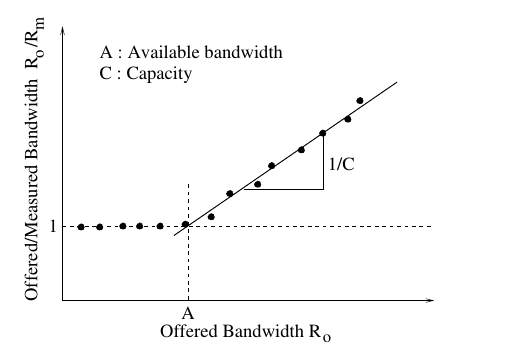
\includegraphics[scale=0.4]{TOPP.png}
		\caption{Approximation de A avec TOPP}
	\end{figure}
\end{frame}

\section{Taxonomie des outils de mesure}
\begin{frame}{Taxonomie des outils de mesure}

\end{frame}


\end{document}
%%% Local Variables: 
%%% mode: latex
%%% TeX-master: t
%%% End: 
\grid
\grid
